	\documentclass[brazil, a4paper]{article}
\usepackage{graphicx}
\usepackage[T1]{fontenc}
\usepackage[utf8]{inputenc}
\usepackage{lmodern}
\usepackage{babel}
\usepackage{url}
\usepackage{xcolor}
\usepackage{textcomp}
\usepackage{listingsutf8}
\usepackage{amsmath}

\lstset{inputencoding=utf8/latin1}

\lstset{language=Python,
	             basicstyle=\footnotesize,
	             numbers=left,
	             numberstyle=\footnotesize,
	             frame=shadowbox,
	             tabsize=2,
	             rulesepcolor=\color{blue},
	             showspaces = false, 
		     showstringspaces = false,
	             showtabs = false,
	             }
\begin{document}


\title{Relatório Final - Simulação Visual do Algoritmo Perceptron}
\author{Pedro Paulo Vezzá Campos \hfill 7538743\\
		Camila Fernandez Achutti \hfill 6795610}
\date{\today}

\maketitle


\section{Proposta escolhida}

O grupo optou pela proposta 2, animação de algoritmos de aprendizagem
computacional. O algoritmo implementado e simulado visualmente foi o Perceptron.

\section{Sobre o problema de aprendizagem}

\subsection{PERCEPTRON}

O algoritmo Perceptron foi inventado em 1957 no Cornell Aeronautical Laboratory
por Frank Rosenblatt. Ele é um classificador supervisionado linear. Ou seja,  a
partir de um conjunto de dados de treinamento, o algoritmo ajusta uma função
linear que será utilizada para a classificação de novas instâncias de teste.

Na sua versão de camada única, é capaz de classificar instâncias de duas classes
distintas, mapeando entradas $x$ para valores de saída $f(x)$ (valores
binários simples) através da função.

$$ f(x) = \begin{cases}1 & \text{se }w \cdot x + b > 0\\0 & \text{senão}\end{cases} $$

Onde $x$ e $w$ são vetores e $w \cdot x$ é o produto escalar. $b$ é a
`inclinação', um termo constante que não depende de qualquer valor de
entrada. Sua principal característica e limitação é que apenas possui  resultados
satisfatórios para a classificação de conjuntos linearmente separáveis.

Assim, instâncias interessantes para o classificador são conjuntos de dados que
podem ou não ser classificados utilizando uma reta para dividir as categorias
de elementos. O caso clássico de conjunto não linearmente separável é a
função ou-exclusivo (XOR). Dentro dos problemas linearmente separáveis,
é interessante considerar casos em que os pontos de dados estão muito ou
pouco separados para verificar a eficiência do classificador.

Neste trabalho implementamos o perceptron para dimensão arbitrária d $\ge$ 2.

\section{Interface Gráfica}

Foi desenvolvida em 2D, ainda que a dimensão $d$ seja maior que 2. Vamos sempre
fazer a representação somente de 2 delas.

A implementação será feita em python e a plotagem será feita usando PyLab e a
interface do usuário usando PyGTK.

A entrada pode ser efetuada de 3 maneiras diferentes:
\begin{itemize}

	\item marcar os pontos no canvas através de clique (opção disponível somente
	para dimensão $d$ igual a 2),

	\item ler de um arquivo de entrada,

	\item gerar pontos de forma aleatória.

\end{itemize}

Com o dataset de entrada o algoritmo de aprendizagem entra em jogo e usa os
pontos de amostragem como um conjunto de treinamento para tentar descobrir qual
é a linha mais adequada para realizar a classificação.

A animação mostra como o algoritmo evolui e quais são os ajustes feitos para
alcançar o resultado final.

A ferramenta de animação terá as seguintes funcionalidades básicas:
\begin{itemize} 
	
	\item Seleção do modo de entrada: Arquivo, Sorteio, Clique;
	
	\begin{itemize}
		
		\item Arquivo: serão necessários a submissão de dois arquivos
		diferentes, um de dados de treino e outro de testes. Ambos são arquivos
		CSV onde o número de colunas deve ser a dimensão escolhida mais uma
		unidade para designação da classe de cada amostra (-1 ou 1).
		
		\item Sorteio: dados aleatórios são gerados, somente com o controle de
		serem gerados dois conjuntos linearmente separáveis. Esse conjuntos são
		gerados por uma distribuição uniforme.
		
		\item Clique: na primeira janela que for aberta serão marcados os pontos
		de treinamento. Para diferenciar uma classe da outra utilizamos os
		botões direito e esquerdo do mouse. Assim que todos os dados de
		treinamento tiverem sido desenhados, o usuário fecha a janela de
		marcação e outra janela se abrirá para marcação dos dados de teste.
		ATENÇÃO: essa opção de entrada somente está disponível para dimensão
		$d$ = 2.

	\end{itemize}

	\item Botão de `TREINAR' para que o algoritmo comece a rodar, ao final do
	algoritmo ele pode ser novamente apertado para que o treinamento seja
	refeito;
	
	\item Botão `TESTAR' para que o conjunto de teste seja plotado e o resultado
	possa ser validado pelo usuário;
	
	\item Possibilidade de  ajustar o valor de $\eta$ (taxa de aprendizagem,
	\texttt{eta} no programa) para controlar a rapidez com que o perceptron
	aprende;
	
	\item Definição do número máximo de iterações, onde uma iteração representa
	a atualização do vetor de pesos a cada ponto que é analisado, sendo assim,
	se a reta inicial arbitrária for correta, encontramos a solução em 0
	iterações do algoritmo.
	
	\item Definição do número de dimensões dos dados de entrada e
	consequentemente do algoritmo perceptron.

\end{itemize}

A taxa de aprendizagem é a que dimensiona o vetor de treinamento antes de ser
adicionado ao vetor de peso durante as atualizações. Experimente valores
diferentes, se quiser, valores maiores afetará a taxa de convergência, mas não a
própria convergência.

O número de iterações é colocado de modo que o algoritmo não será executado para
sempre se os vetores de entrada não são separáveis.

Normalmente, um valor maior de $\eta$ fará com que ele encontre uma solução mais
rapidamente, mas pode causar a perda de soluções de casos difíceis. E a
definição do número máximo de iteração garante que o algoritmo vai ter fim,
ainda que não encontre um solução de erro global nulo.

A sequência esperada do usuário e da animação é a seguinte:

\begin{enumerate}
	
	\item seleção do modo de entrada
	
	\item plotagem do conjunto de treinamento 
	
	\item clique do usuário no botão `TREINAR'
	
	\item plotagem das retas que o algoritmo encontrou durante a execução 
	
	\item clique no botão `TESTAR' para que o conjunto de teste seja plotado e o
	algoritmo possa ser avaliado pelo usuário.

\end{enumerate}

O botão de 'TREINAR' pode ser usado para que o algoritmo refaça o treinamento
com os mesmos dados, mas com a possibilidade de trocar os parâmetros
\texttt{eta} e \texttt{máximo de iterações}.

\section{Cronograma}

Na tabela a seguir estão listadas as tarefas cumpridas para o projeto de MAC0460
de 2013:

\begin{table}[h]
    \begin{tabular}{|p{5cm}|c|c|c|c|}
    \hline
    Atividade                                                       & setembro & outubro & novembro & dezembro \\ \hline
    Implementar o Perceptron                                        & X        & ~       & ~        & ~        \\
    Buscar na Internet e testar entradas interessantes como exemplo & X        & X       & ~        & ~        \\
    Implementar a interface gráfica                                 & X        & X       & X        & ~        \\
    Escrever o relatório parcial                                    & ~        & X       & ~        & ~        \\ 
    Escrever o relatório final                                      & ~        & ~       & X        & X        \\ \hline
    \end{tabular}
    \caption{Cronograma das tarefas a serem realizadas no semestre}
\end{table}

O cronograma proposto foi cumprido e não sofreu qualquer alteração durante o
decorrer do trabalho.

\section{O que foi feito}


\subsection{Estudo e implementação do algoritmo perceptron em Python}

Realizamos um estudo detalhado do funcionamento do algoritmo  e realizamos a
seguinte implementação em Python:

\lstinputlisting{perceptron.py}


\subsection{Busca de exemplos interessantes para teste da animação}

\begin{description}

    \item[XOR] O exemplo aqui é a função XOR. Nele não é possível traçar uma
	única reta (função linear) tal que divida o plano de maneira que as saídas com
	valor 0 ficam situadas de um lado da reta e as com valor 1 do outro. Entretanto,
	este problema pode ser solucionado com a criação de uma camada intermediária na
	rede e graficamente com uma estrutura em três (ou mais) dimensões.
	
		\begin{table}[h]
			\centering
			\begin{tabular}{|c|c|c|}
			\hline
			x1 & x2 & u \\ \hline
			0 & 0 & 0 \\
			0 & 1 & 1 \\
			1 & 0 & 1 \\
			1 & 1 & 0 \\ \hline
			\end{tabular}
			\caption{Conjunto de treinamento do exemplo XOR}
		\end{table}
		
	\item[Violeta para exportação]
	
	Neste exemplo temos que classificar violetas para serem importadas e as que
	vão ficar no mercado.
	
	As violetas são classificadas de acordo com uma escala de intensidade de cor
	que vai de 1 a 8 e outra escala de textura que vai de 1 a 5.
	
	Definimos que a classe 1 é a de exportação e a classe 2 é a para mercado
	interno e temos o seguinte conjunto de teste:

	\begin{table}[h]
			\centering
			\begin{tabular}{|c|c|c|}
			\hline
			cor & textura & classe \\ \hline
			4 &5 & 1 \\
			5 & 4 & 1 \\
			6 & 3 & 1 \\
			7 & 1 & 1 \\
			8 & 2 & 1 \\
			1 & 3 & 2 \\
			1 & 5 & 2 \\
			2 & 2 & 2 \\
			3 & 4 & 2 \\
			4 & 2 & 2 \\ \hline
			\end{tabular}
			\caption{Conjunto de treinamento do exemplo das violetas}
		\end{table}

	\begin{table} [h]
			\centering
			\begin{tabular}{|c|c|c|}
			\hline
			cor & textura & classe \\ \hline
			5 & 1 & 1 \\
			5 & 3 & 2 \\
			6 & 2 & 1 \\ \hline
			\end{tabular}
			\caption{Conjunto de teste do exemplo das violetas}
		\end{table}


\subsection{Implementação da interface gráfica}

A interface gráfica já desenvolvida se restringe a exibição dos pontos de
treinamento e teste e das linhas obtidas durante o treinamento.

Assim que o programa rodar ele abre uma janela como ilustrada abaixo:

\begin{figure}[!htb]
\centering
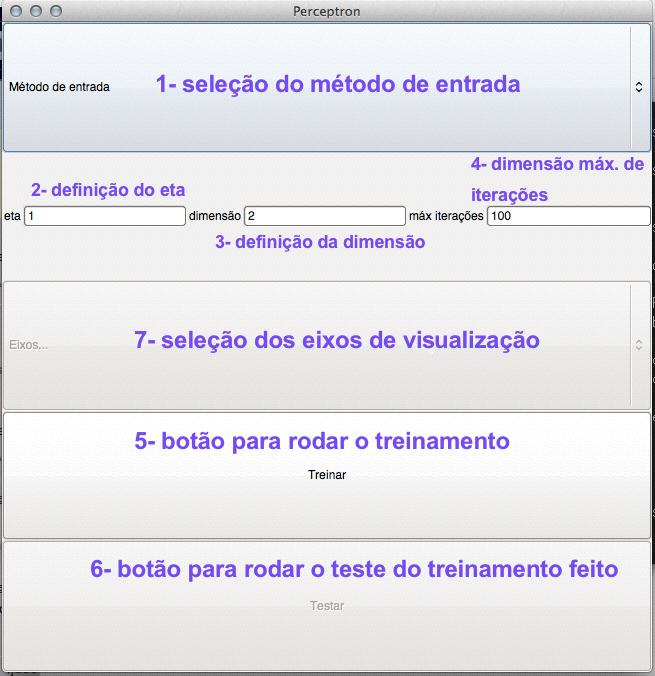
\includegraphics[scale=0.35]{interfaceInicial.jpg}
\caption{Interface com o usuário.}
\end{figure}

A interface com o usuário já está implementada para suportar sequências de
cliques errados, como visto abaixo:


\begin{figure}[!htb]
\centering
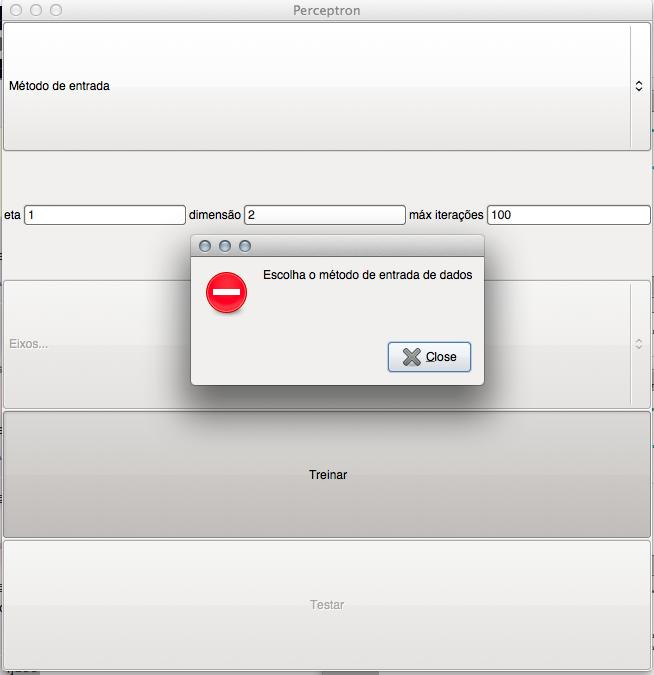
\includegraphics[scale=0.35]{erro.jpg}
\caption{Interface com o usuário.}
\end{figure}

Se escolhermos sortear os dados o nosso aplicativo se comporta da seguinte
maneira representada pela sequência de fotos abaixo:

\begin{figure}[!htb]
\centering
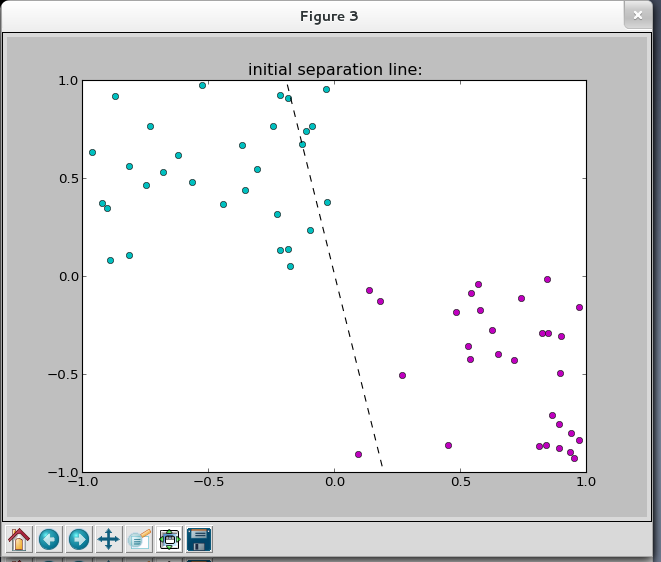
\includegraphics[scale=0.32]{ex1-1.png}
\caption{Situação inicial do exemplo 1, onde uma reta arbitrária foi sorteada.}
\end{figure}

\newpage

\begin{figure}[!htb]
\centering
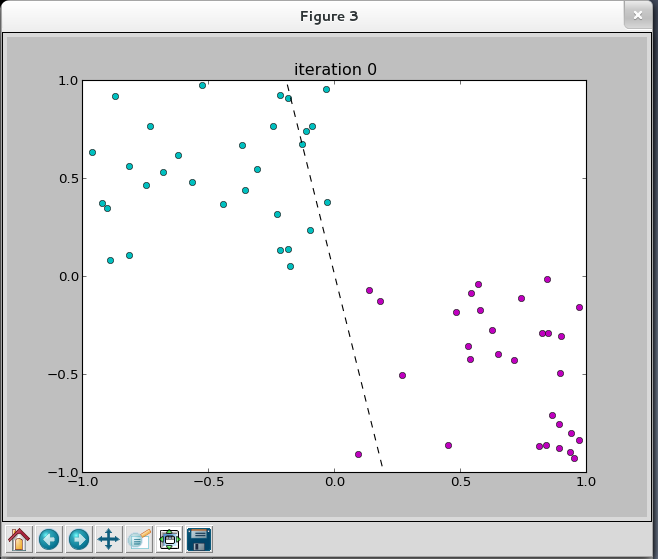
\includegraphics[scale=0.42]{ex1-2.png}
\caption{Começa a execução do algoritmo para o exemplo 1.}
\end{figure}

\begin{figure}[!htb]
\centering
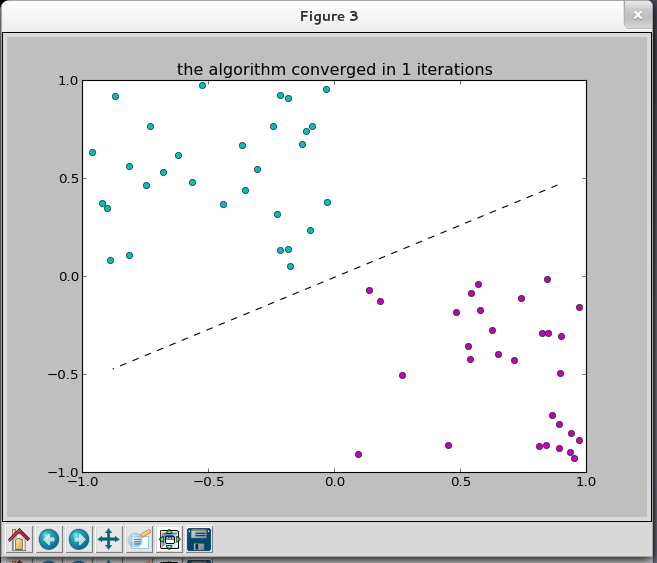
\includegraphics[scale=0.42]{ex1-3.png}
\caption{Fim do algoritmo, reta classificadora foi encontrada no exemplo 1.}
\end{figure}

Agora queremos mostrar como é feito o teste, que é quando o usuário clica no
botão TESTAR. Lembrando que só será valido se ele já tiver realizado o treino.

\newpage

\begin{figure}[!htb]
\centering
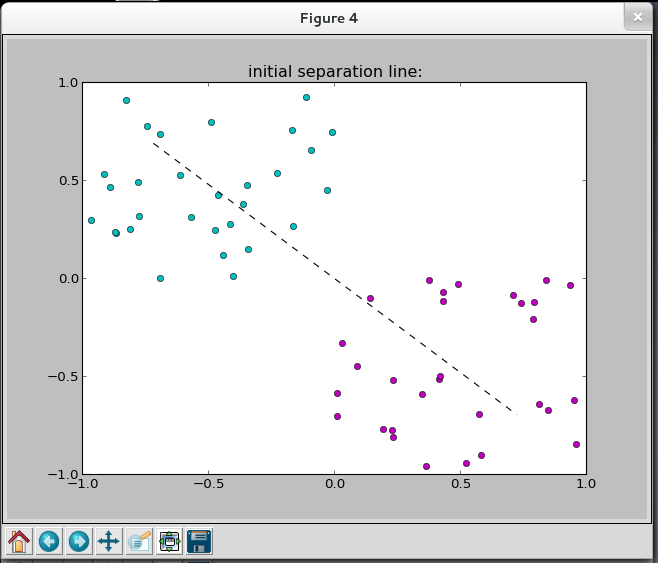
\includegraphics[scale=0.42]{ex2-1.png}
\caption{Situação inicial do exemplo 2, onde uma reta arbitrária foi sorteada.}
\end{figure}

\begin{figure}[!htb]
\centering
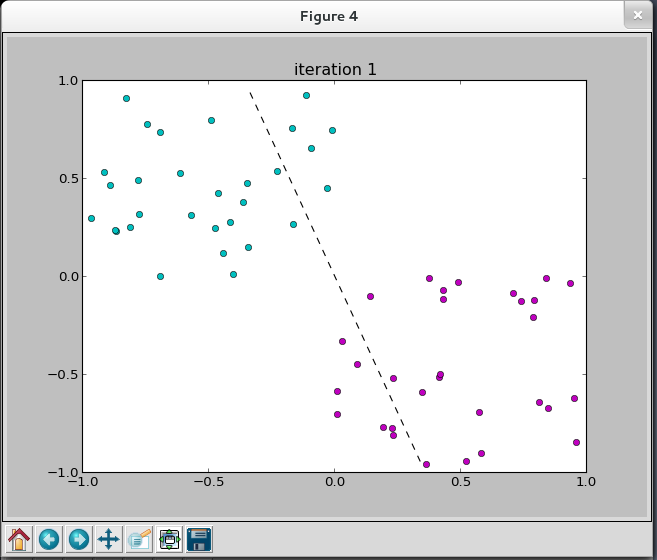
\includegraphics[scale=0.42]{ex2-2.png}
\caption{Começa a execução do algoritmo para o exemplo 2.}
\end{figure}

\newpage

\begin{figure}[!htb]
\centering
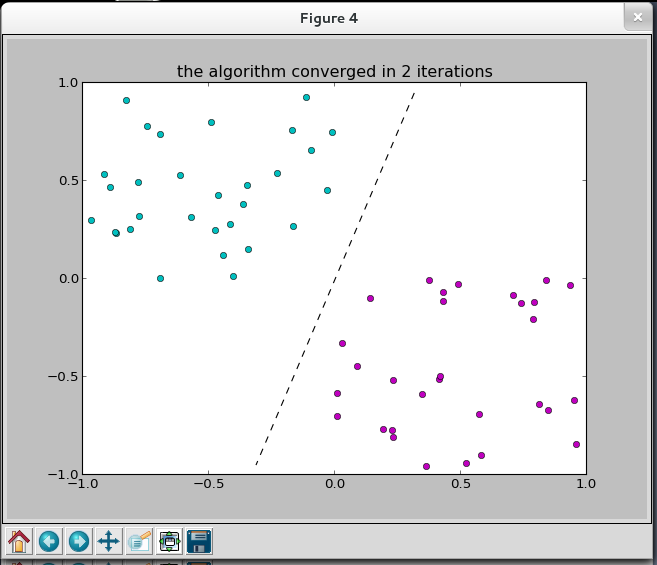
\includegraphics[scale=0.42]{ex2-3.png}
\caption{Fim do algoritmo, reta classificadora foi encontrada para o exemplo 2.}
\end{figure}

Agora se o usuário apertar o botão TESTAR os dados de treino serão retirados do
gráfico e os dados de teste serão colocados conforme ilustrado nas imagens
abaixo:

\begin{figure}[!htb]
\centering
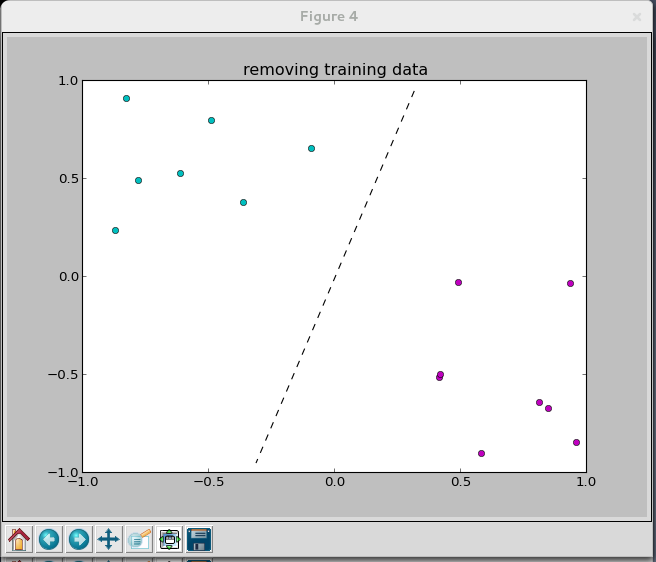
\includegraphics[scale=0.42]{ex2-t1.png}
\caption{Remoção dos dados de treino.}
\end{figure}

\newpage

\begin{figure}[!htb]
\centering
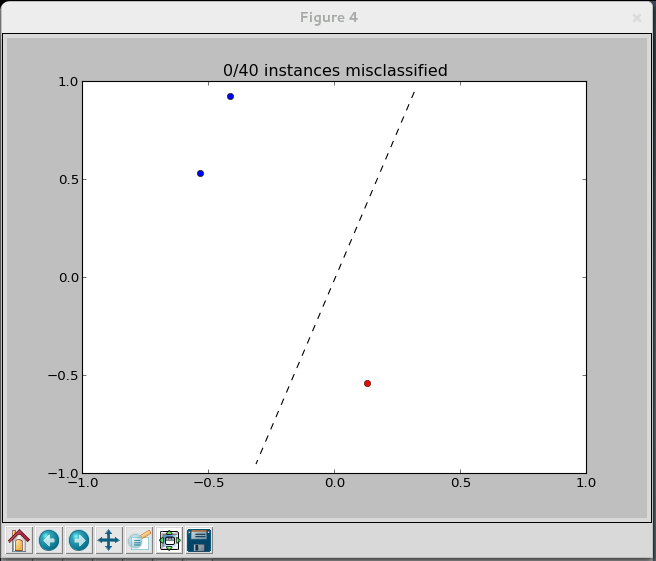
\includegraphics[scale=0.42]{ex2-t2.png}
\caption{Exibição dos dados de teste.}
\end{figure}

\begin{figure}[!htb]
\centering
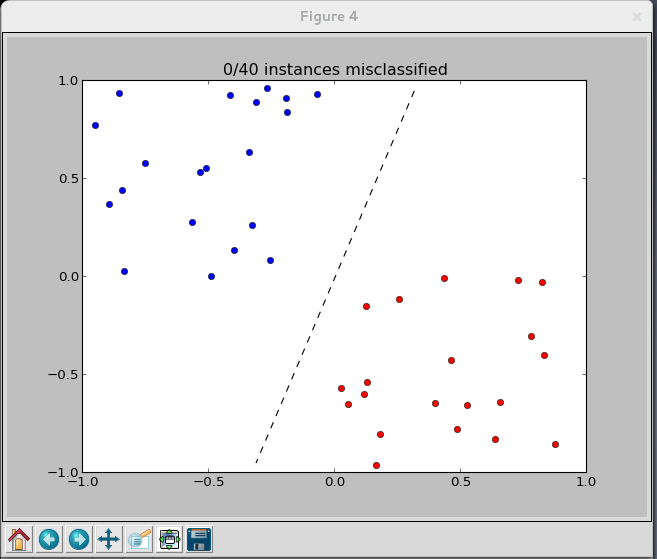
\includegraphics[scale=0.42]{ex2-t3.png}
\caption{Fim do teste para o exemplo 2.}
\end{figure}

Neste caso apresentado acima temos um treinamento bem sucedido. Agora vamos
ilustrar uma caso de treinamento mal-sucedido. Para isso alteramos o eta para um
valor baixo para que a taxa de aprendizado fosse bem baixa e limitamos o número
de iterações para 1. O resultado obtido está ilustrado abaixo:


\begin{figure}[!htb]
\centering
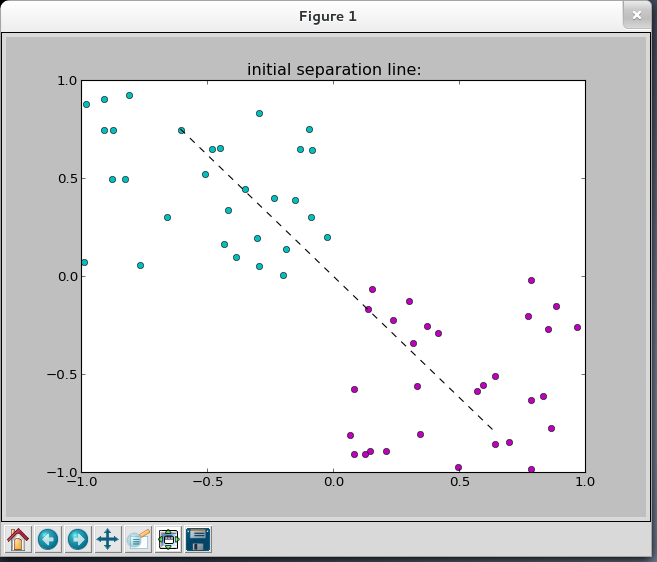
\includegraphics[scale=0.42]{ex3-1.png}
\caption{Exibição dos dados de teste.}
\end{figure}

\begin{figure}[!htb]
\centering
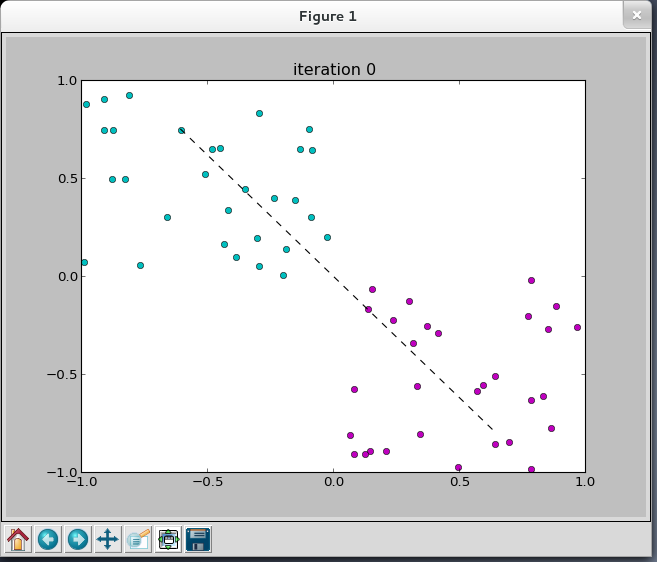
\includegraphics[scale=0.42]{ex3-2.png}
\caption{Fim do teste para o exemplo 2.}
\end{figure}

\newpage

\begin{figure}[!htb]
\centering
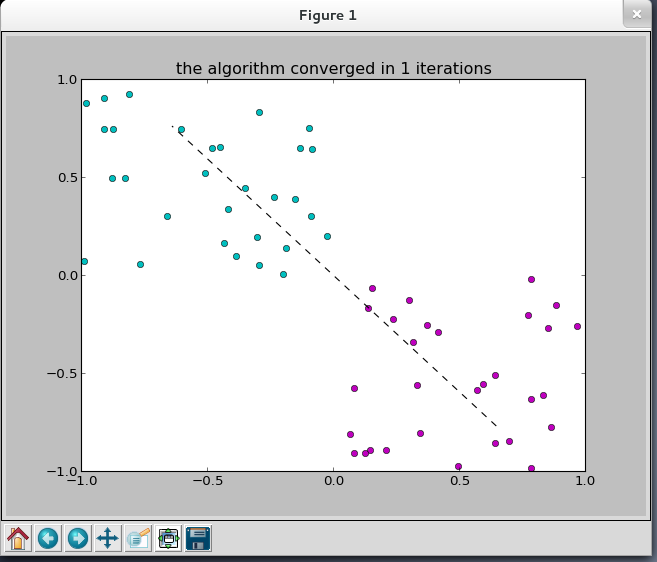
\includegraphics[scale=0.42]{ex3-3.png}
\caption{Exibição dos dados de teste.}
\end{figure}

\begin{figure}[!htb]
\centering
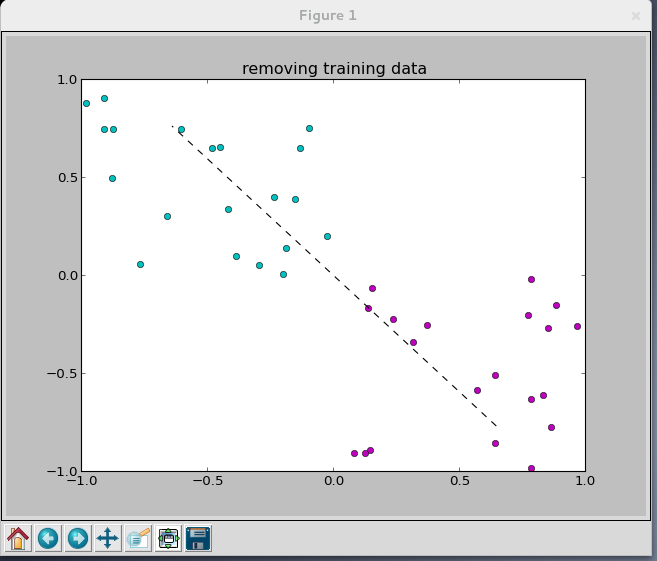
\includegraphics[scale=0.42]{ex3-4.png}
\caption{Fim do teste para o exemplo 2.}
\end{figure}

\newpage
\begin{figure}[!htb]
\centering
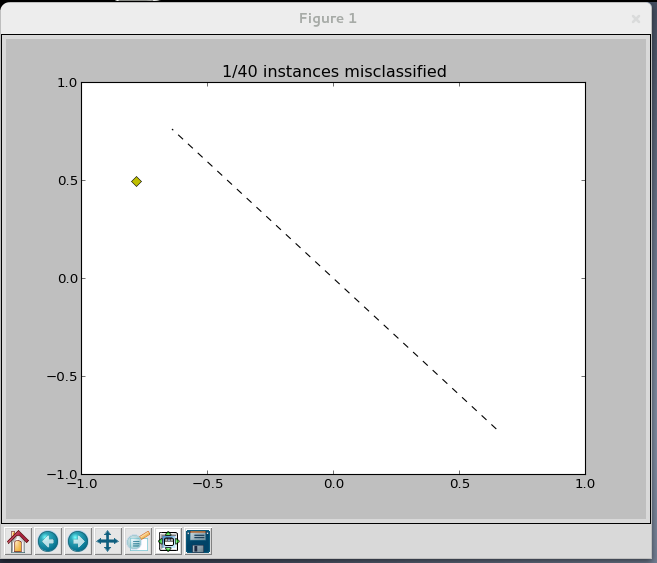
\includegraphics[scale=0.42]{ex3-t1.png}
\caption{Exibição dos dados de teste.}
\end{figure}

\begin{figure}[!htb]
\centering
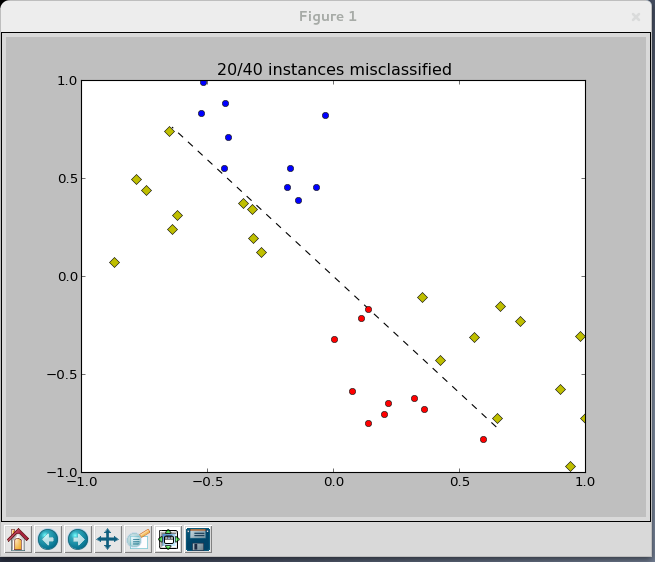
\includegraphics[scale=0.42]{ex3-t2.png}
\caption{Fim do teste para o exemplo 3.}
\end{figure}


Aqui esclarecemos que o diamante amarelo representa os dados de teste mal classificados de ambas as amostras.

Depois que o algoritmo terminou de processar o treinamento ou o teste do conjunto de dados, a combobox de seção dos eixos que devem ser exibidos fica habilitada e podemos observar o resultado por todas as perpectivas possíveis. Por exemplo como visto abaixo na sequência de imagens para o mesmo resultado de um treinamento em dimensão 3:
\begin{itemize}
\item Eixos 1 e 2:
\begin{figure}[!htb]
\centering
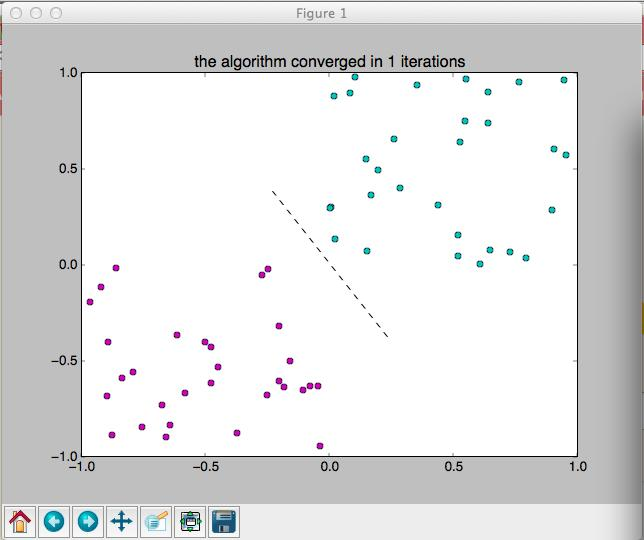
\includegraphics[scale=0.4]{eixo12.jpg}
\caption{Fim do teste para o exemplo 3.}
\end{figure}

\item Eixos 1 e 3:
\begin{figure}[!htb]
\centering
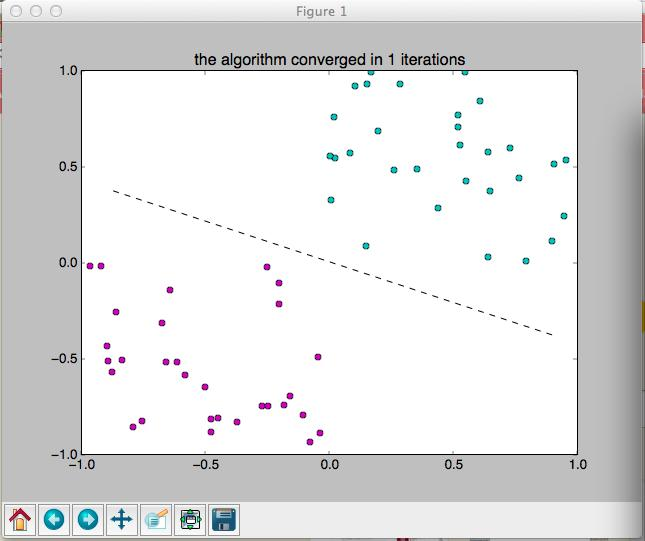
\includegraphics[scale=0.35]{eixo13.jpg}
\caption{Fim do teste para o exemplo 3.}
\end{figure}

\item Eixos 2 e 3:
\begin{figure}[!htb]
\centering
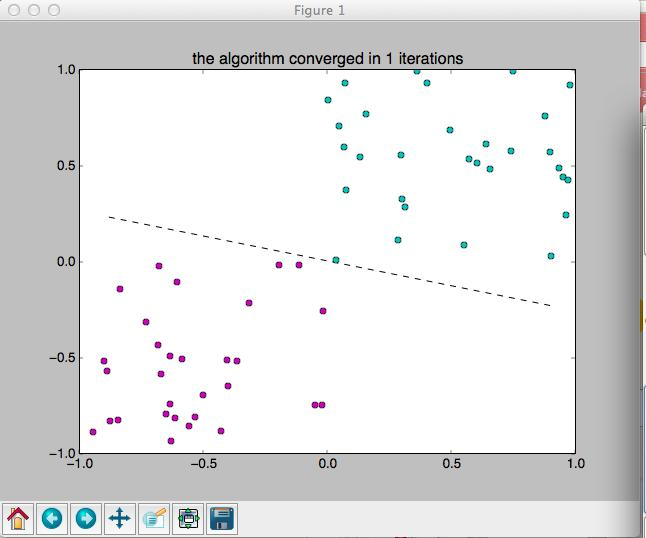
\includegraphics[scale=0.4]{eixo23.jpg}
\caption{Fim do teste para o exemplo 3.}
\end{figure}
\end{itemize}

É possível também realizar a entrada de dados por arquivos externos. Devem ser produzidos e carregados dois arquivos separados um de treinamento e outro de teste, ambos no formato CSV com o seguinte padrão: \texttt{x1, x2, ..., xn, classe}, onde a classe é 1 ou -1 e n é a dimensão escolhida. A entrada pode ainda ser gerada por clique de mouse, onde cliques com o botão esquerdo representam uma classe e cliques com botão direito representam outra classe.
\end{description} 


\section{Possíveis trabalhos futuros}

\begin{itemize}
\item Representação 3D do resultado para dimensões maiores que 2
\item Aumentar o número de classes possíveis.
\end{itemize}  


\section{Parte Subjetiva}

Nesta seção os alunos fazem um balanço da disciplina MAC0460, êxitos e
frustrações enfrentadas durante o semestre:

\subsection{O que deu certo}

\begin{description}
	\item[Exercícios Práticos] Aplicar os algoritmos em programas reais e ver 
	o resultado, muitas vezes visual, incentiva bastante a experimentação e
	motiva o aluno a buscar a interpretação dos resultados que está recebendo.

    \item[Projeto Final] O projeto final da disciplina aliou a aplicação de
	conceitos vistos em aula com a geração de um produto de software potencialmente
	útil para outros alunos de Aprendizagem Computacional. O contato com alunos
	da pós-graduação é bastante enriquecedor durante as apresentações finais.
	Foi possível ver a grande gama de aplicações que os tópicos estudados em
	sala de aula permitem desenvolver.

\end{description}

\subsection{O que não deu certo}

\begin{description}

	\item[Comprometimento dos alunos de graduação] A maioria dos alunos de graduação que cursa
	MAC0460 são alunos de quarto ano ou posterior. No caso do nosso
	grupo, e de ouro ambos os membros da equipe estavam cumprindo iniciações
	científicas juntamente com seus respectivos TCCs. Conciliar todas as
	atividades acadêmicas foi algo extremamente difícil aos alunos e infelizmente
	nossa participação em sala de aula foi menor que o desejável.

\end{description}

\subsection{O que pode melhorar}
\begin{description}

	\item[Descrição da disciplina] MAC0460 exigiu uma maturidade matemática maior
	que o esperado pelo grupo. No início do semestre, já esperávamos um curso
	instrumental, porém com menor profundidade do que o que foi mostrado. Isto
	não é um problema por si só. Apenas seria interessante que os alunos fossem
	melhor avisados do que devem esperar no curso. Uma possibilidade seria
	disponibilizar as notas de aula para que quem estivesse interessado em
	MAC0460 soubesse como os tópicos são abordados. Outra ideia é a
	disponibilização de um vídeo curto no qual a professora descreve a
	disciplina em mais detalhes. O Projeto Apoio BCC, orientado pelo Prof.
	Coelho está disponível para operacionalizar a produção do vídeo.

	\item[Exercícios programa] EPs, em substituição a algumas listas de exercício,
	poderiam ser aplicados aos alunos para fixar os conceitos vistos em aula.
	Programar para resolver algum problema proposto tende a ser mais divertido a
	um aluno de Computação que resolver uma lista de exercícios em papel.

\end{description}


\section{Bibliografia}
\begin{itemize}
\item \url{http://computing.dcu.ie/~humphrys/Notes/Neural/single.neural.html}
\item \url{http://eecs.wsu.edu/~cook/ai/lectures/applets/perceptron/}
\item \url{http://matplotlib.org/}
\item \url{http://www.pygtk.org/}
\end{itemize}
\end{document}

